\documentclass[tikz,border=3pt]{standalone}
\pdfminorversion=5
\usepackage{xcolor}
\usetikzlibrary{arrows.meta,calc,positioning}

\definecolor{ink}{HTML}{1F2937}
\definecolor{muted}{HTML}{64748B}
\definecolor{grid}{HTML}{D4DEE9}
\definecolor{blue}{HTML}{2F6FA7}
\definecolor{orange}{HTML}{E58B2A}
\definecolor{green}{HTML}{2E8B57}
\definecolor{greenSoft}{HTML}{E8F5EE}

\begin{document}
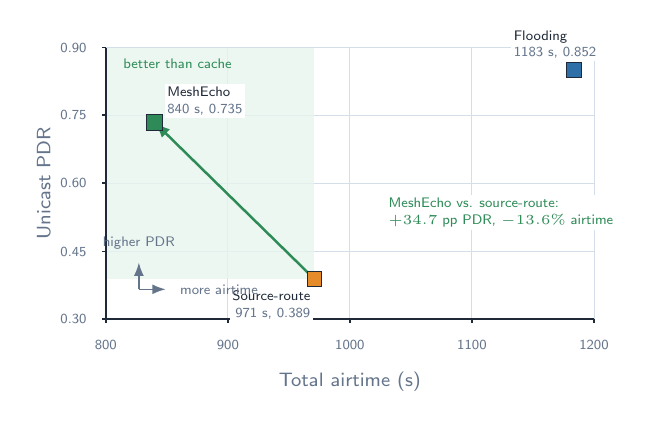
\begin{tikzpicture}[
    font=\sffamily\scriptsize,
    axis/.style={draw=ink, line width=0.65pt},
    gridline/.style={draw=grid, line width=0.35pt},
    point/.style={line width=0.35pt, draw=ink},
    label/.style={font=\sffamily\tiny, text=ink, fill=white, inner sep=1pt},
    note/.style={font=\sffamily\tiny, text=muted},
    arrow/.style={-{Latex[length=2.0mm]}, draw=green, line width=0.9pt}
]

% Plot area: x = total airtime, y = unicast PDR.
\def\xmin{800}
\def\xmax{1200}
\def\ymin{0.30}
\def\ymax{0.90}
\def\W{6.2}
\def\H{3.45}

\coordinate (O) at (0,0);
\coordinate (TL) at (0,\H);
\coordinate (BR) at (\W,0);

% Grid and ticks.
\foreach \x/\lab in {0/800,1.55/900,3.10/1000,4.65/1100,6.20/1200} {
    \draw[gridline] (\x,0) -- (\x,\H);
    \draw[axis] (\x,0) -- ++(0,-0.045);
    \node[note, anchor=north] at (\x,-0.15) {\lab};
}
\foreach \y/\lab in {0/0.30,0.86/0.45,1.73/0.60,2.59/0.75,3.45/0.90} {
    \draw[gridline] (0,\y) -- (\W,\y);
    \draw[axis] (0,\y) -- ++(-0.045,0);
    \node[note, anchor=east] at (-0.12,\y) {\lab};
}

% Improvement region relative to source-route cache.
\path[fill=greenSoft, opacity=0.78] (0,0.51) rectangle (2.65,\H);
\node[note, anchor=west, text=green] at (0.10,\H-0.20) {better than cache};

% Axes.
\draw[axis] (0,0) -- (0,\H);
\draw[axis] (0,0) -- (\W,0);
\node[font=\sffamily\scriptsize, text=muted, anchor=north] at (\W/2,-0.55) {Total airtime (s)};
\node[font=\sffamily\scriptsize, text=muted, rotate=90, anchor=south] at (-0.58,\H/2) {Unicast PDR};

% Data coordinates.
\coordinate (Flood) at (5.94,3.17);
\coordinate (Cache) at (2.65,0.51);
\coordinate (Calm) at (0.62,2.50);

% Reference movement from source-route cache to MeshEcho.
\draw[arrow] (Cache) -- (Calm);
\node[label, anchor=north west, align=left, text=green] at (3.55,1.58)
    {MeshEcho vs. source-route:\\$+34.7$ pp PDR, $-13.6\%$ airtime};

% Points.
\node[point, fill=blue, rectangle, minimum size=5.4pt, inner sep=0pt] at (Flood) {};
\node[point, fill=orange, rectangle, minimum size=5.4pt, inner sep=0pt] at (Cache) {};
\node[point, fill=green, rectangle, minimum size=5.8pt, inner sep=0pt] at (Calm) {};

% Direct labels.
\node[label, anchor=south west, align=left] at ($(Flood)+(-0.80,0.10)$)
    {Flooding\\{\color{muted}1183 s, 0.852}};
\node[label, anchor=north east, align=right] at ($(Cache)+(-0.01,-0.11)$)
    {Source-route\\{\color{muted}971 s, 0.389}};
\node[label, anchor=south west, align=left] at ($(Calm)+(0.12,0.05)$)
    {MeshEcho\\{\color{muted}840 s, 0.735}};

% Small orientation cue.
\draw[-{Latex[length=1.7mm]}, draw=muted, line width=0.55pt] (0.42,0.38) -- (0.42,0.72);
\draw[-{Latex[length=1.7mm]}, draw=muted, line width=0.55pt] (0.42,0.38) -- (0.76,0.38);
\node[note, anchor=west] at (0.82,0.38) {more airtime};
\node[note, anchor=south] at (0.42,0.76) {higher PDR};

\end{tikzpicture}
\end{document}
